\section{Natural Language Processing Methodology}
\label{sec:nlp_methodology}

Building on the established causal impact, we now turn to our primary contribution: a comprehensive NLP analysis of how question content, complexity, and focus have evolved in response to ChatGPT's introduction. This section outlines our NLP methodology for detecting and characterizing these changes.

%%%%%%%%%%%%%%%%%%%%%%%%%%%%%%%%%%%%%%%%%%%%%%%%%%%%%%%%%%%%%%%%%%%%%%%%%%%%%%%%%%%%%%%%%%%%%%%%

\subsection{Data Pre-processing}
\textit{[PREPROCESSING PLACEHOLDER - Will detail specific preprocessing steps including tokenization, stopword removal, lemmatization, etc.]}

The resulting word clouds show no immediate clear trend:

\begin{figure}[H]
    \centering
    \begin{subfigure}[b]{0.475\textwidth}
        \centering
        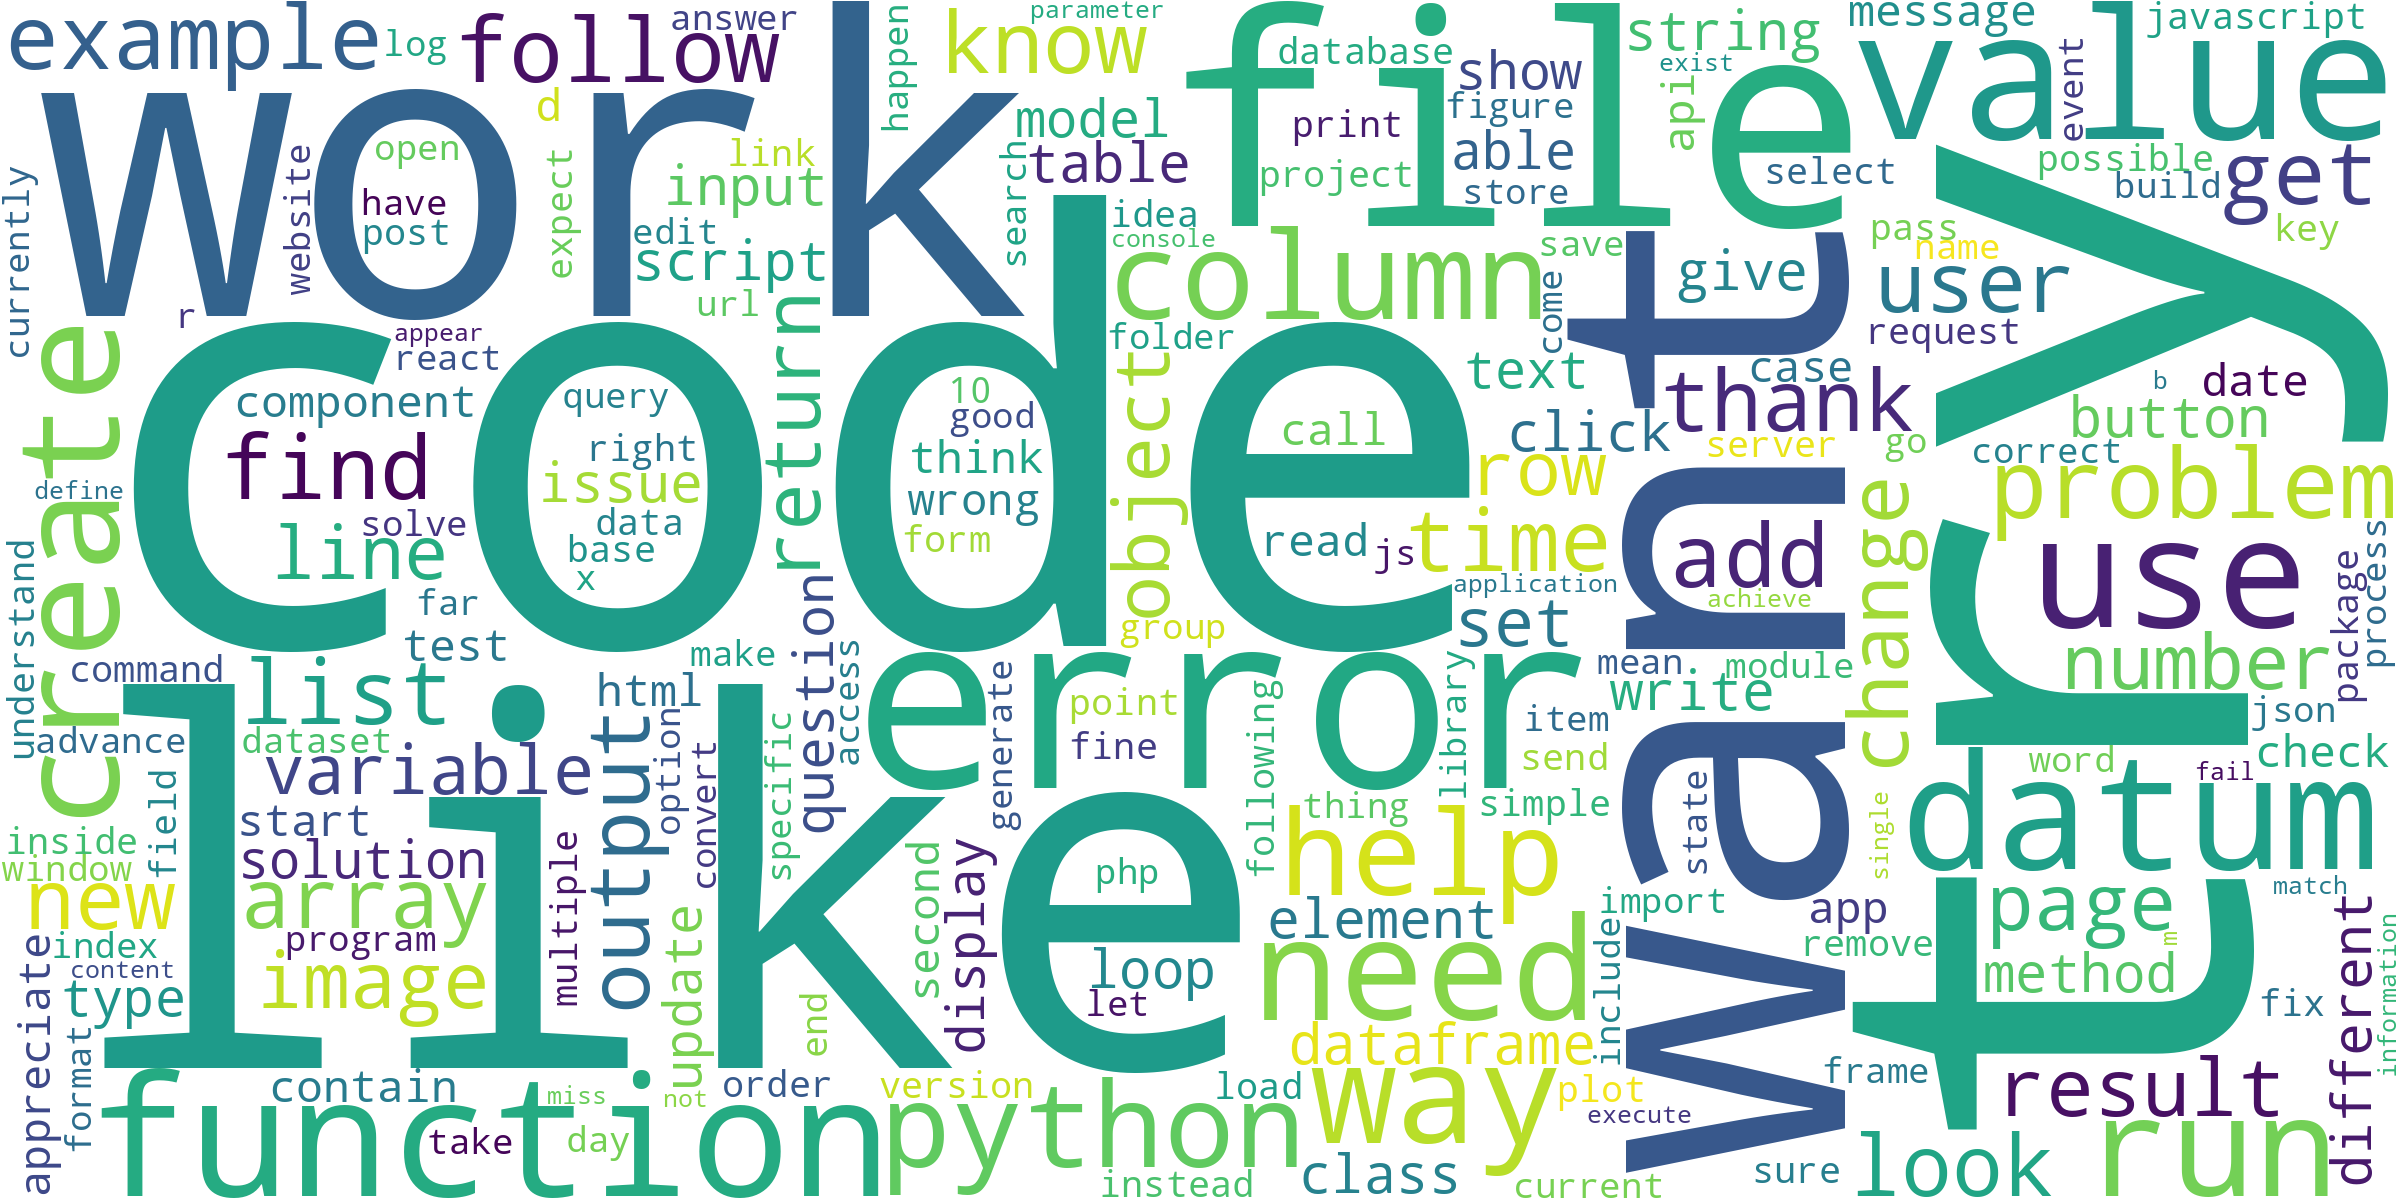
\includegraphics[width=1\linewidth]{imgs/wordclouds/wc_stackoverflow_pre_alphanum.png}
        \caption{Pre-treatment wordcloud}
        \label{fig:prewc}
    \end{subfigure}
    \hfill
    \begin{subfigure}[b]{0.475\textwidth}
        \centering
        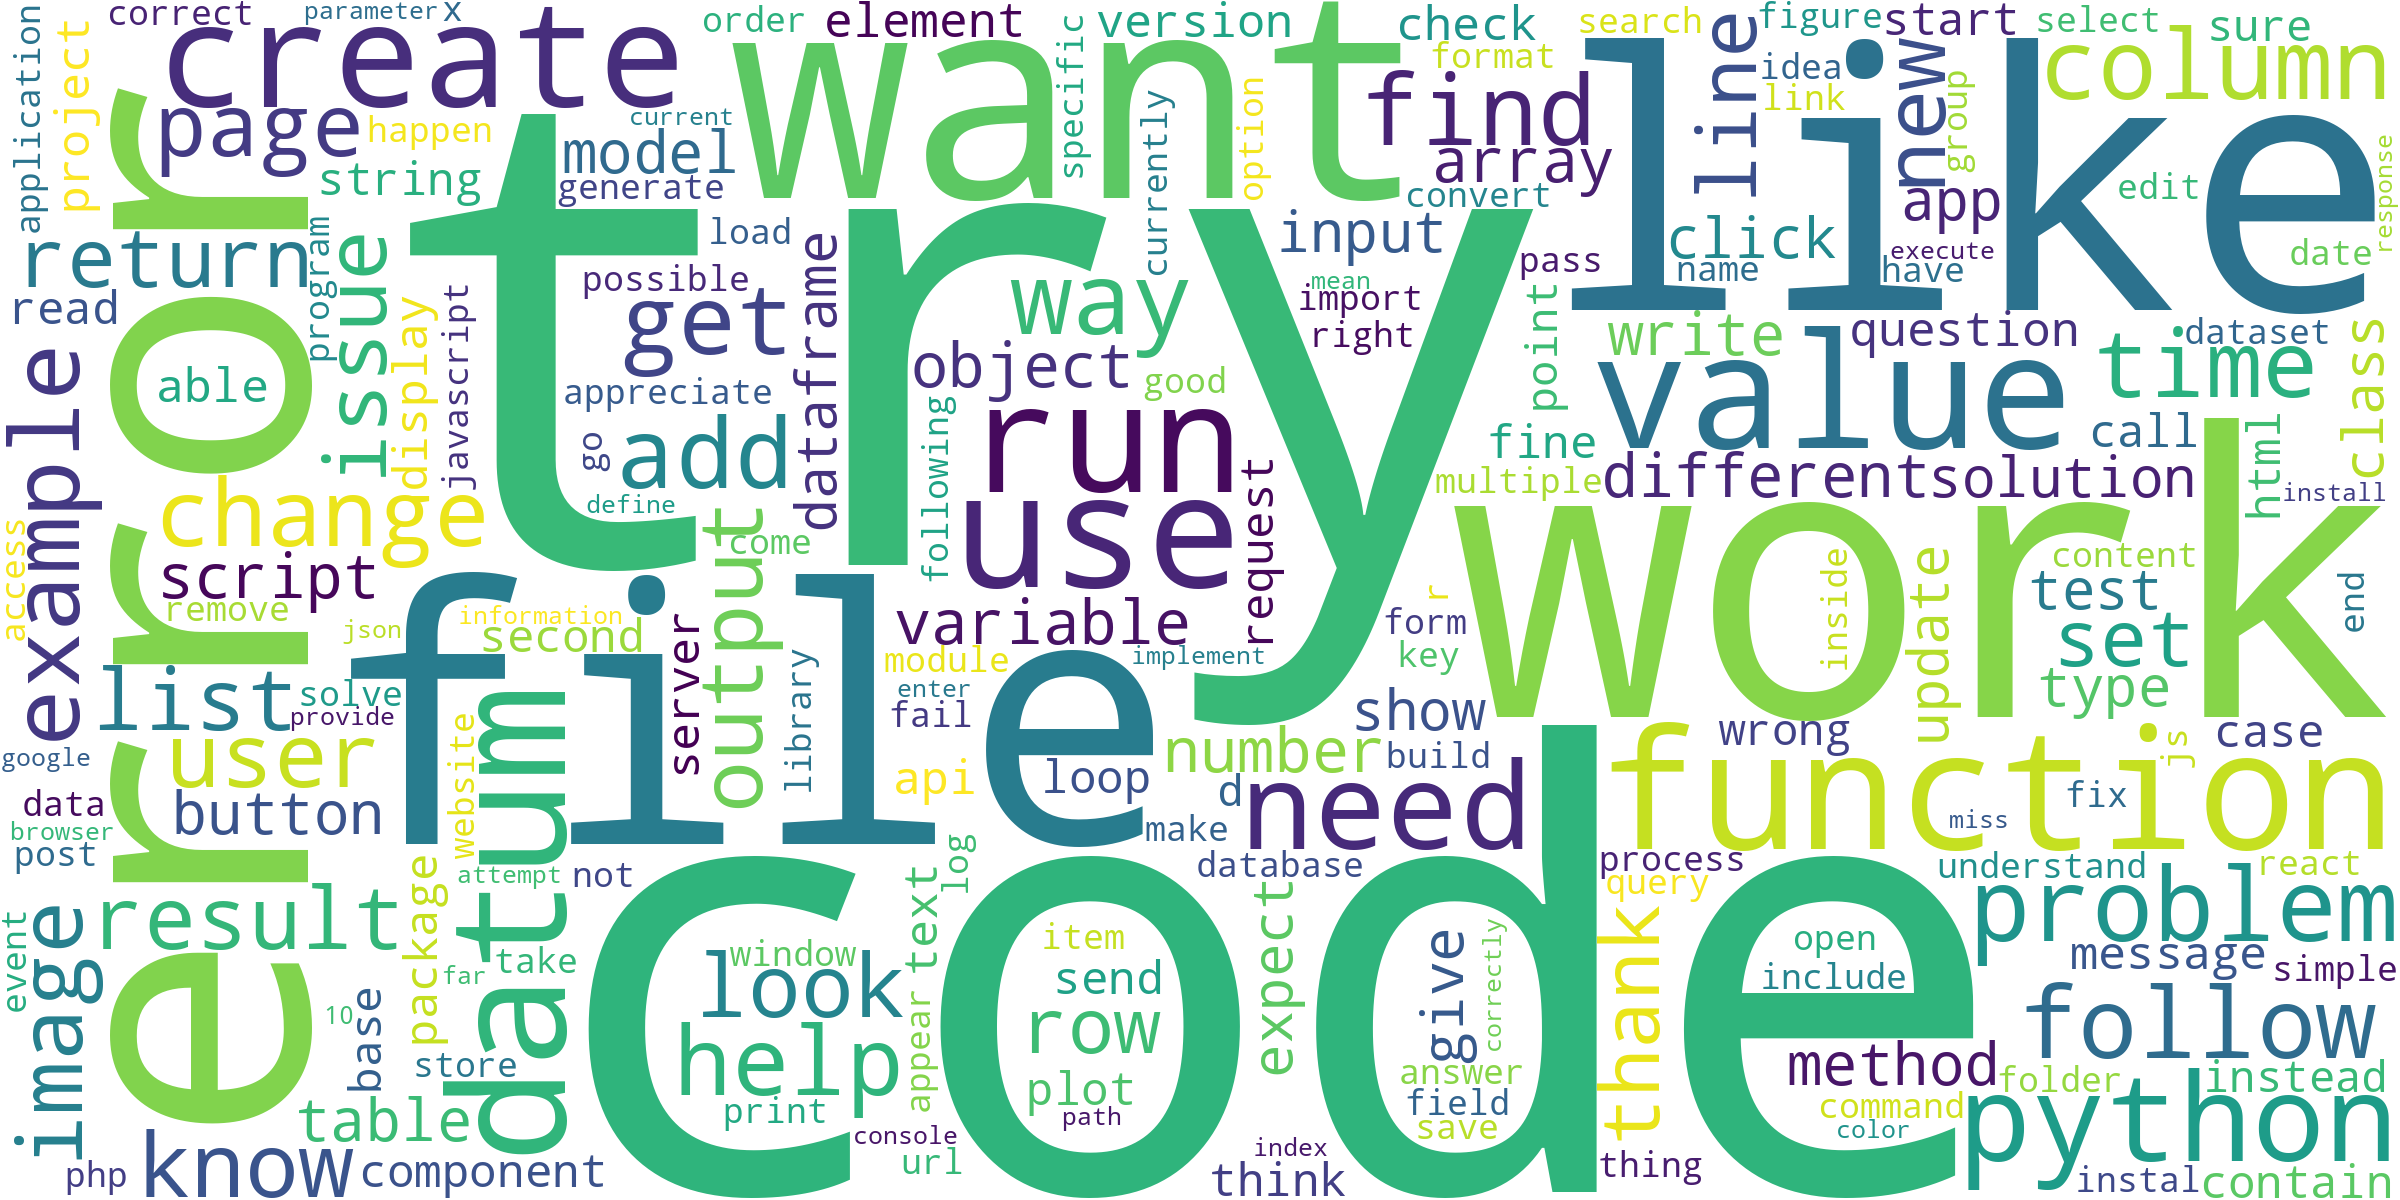
\includegraphics[width=1\linewidth]{imgs/wordclouds/wc_stackoverflow_post_alphanum.png}
        \caption{Post-treatment wordcloud}
        \label{fig:postwc}
    \end{subfigure}
\end{figure}

%%%%%%%%%%%%%%%%%%%%%%%%%%%%%%%%%%%%%%%%%%%%%%%%%%%%%%%%%%%%%%%%%%%%%%%%%%%%%%%%%%%%%%%%%%%%%%%%

\subsection{Complexity Analysis}

We construct a parsimonious complexity score for forum posts which is composed of 4 key elements: (1) title length, (2) body length, (3) number of tags and (4) length of technical expressions (i.e. code, or equation length for the respective forums)\footnote{We used different metrics appropriate to each forum's content: code length was measured for Stack Overflow, Superuser, and Askubuntu, while equation length was used for Mathematics and Physics. This distinction reflects the content patterns in our data, as Physics and Mathematics questions contained code in fewer than 5\% of posts, while the technology-focused forums rarely contained equations.}:

\begin{multline}\label{eq:cscore}
    \text{Complexity Score}_{i,t} = \\ 
    \frac{1}{4} \left( \frac{\text{TagCount}_{i,t} - \mu_{\text{TagCount}}}{\sigma_{\text{TagCount}}} + \frac{\text{TechExprLength}_{i,t} - \mu_{\text{TechExprLength}}}{\sigma_{\text{TechExprLength}}} \right. \\
    \left. + \frac{\text{BodyLength}_{i,t} - \mu_{\text{BodyLength}}}{\sigma_{\text{BodyLength}}} + \frac{\text{TitleLength}_{i,t} - \mu_{\text{TitleLength}}}{\sigma_{\text{TitleLength}}} \right)
\end{multline}

\equationref{eq:cscore} thus shows the complexity score of forum $i$ in time (week) $t$. The reason for choosing this relatively simple score is that questions often use snippets of code or equations. Thus, more sophisticated and established equation or code complexity algorithms become unusable. \tableref{fig:complex} presents the results over time:

\begin{figure}[H]
    \centering
    \includesvg[width=1\linewidth]{imgs/stackoverflow_vs_rest.svg}
    \caption{Treatment vs. Control: Question complexity over time}
    \label{fig:complex}
\end{figure}

%%%%%%%%%%%%%%%%%%%%%%%%%%%%%%%%%%%%%%%%%%%%%%%%%%%%%%%%%%%%%%%%%%%%%%%%%%%%%%%%%%%%%%%%%%%%%%%%

\subsection{Term Frequencies}

Conclusively, and to better understand the nature of the complexity changes identified in our Synthetic DiD analysis, we then examine shifts in term importance using word frequency analysis. \figureref{} shows percentage changes in term importance before and after ChatGPT's introduction.\\

To ensure observed term changes represent genuine shifts rather than random variation, we test statistical significance using bootstrapped confidence intervals and permutation tests ($\alpha = 0.05$) -- terms marked with an asterisk (*) in \figureref{} show statistically significant changes.